\documentclass{beamer}[10]
\usetheme{default}
\usepackage{pgf}
\usepackage[utf8]{inputenc}
\usepackage[brazil]{babel}
\usepackage{beamerthemesplit}
\usepackage{graphics,epsfig, subfigure}
\usepackage{url}
\usepackage{srcltx}
\usepackage{hyperref}



\title[Cobertura Mínima de Vértices]
{\textbf{Uma Heurística para o Problema da Cobertura Mínima de
    Vértices}}
\author[guedesav, dggc]{Bruno Guedes, Daniel Galinkin}

\institute[UFMG] % opcional
{Departamento de Ciência da Computação
\\Universidade Federal de Minas Gerais}

\subject{Teoria de Grafos}

\date{\today}

\begin{document}

   \frame{\titlepage}

   % Mostra um table of contents no inicio de cada subsection:
   \AtBeginSection[] {
     \begin{frame}<beamer>{Sumário}
       \tableofcontents[currentsection,currentsubsection]
     \end{frame}
   }
   \AtBeginSubsection[] {
     \begin{frame}<beamer>{Sumário}
       \tableofcontents[currentsection,currentsubsection]
     \end{frame}
   }

    
\section{Introdução}
\subsection{Definição}
    
\frame{
\frametitle{Definição}
Dado um grafo $G = (V, E)$, uma cobertura de vértices (\textit{CV}) é
    um subconjunto $C \subseteq V \mid \forall e=(a,b) \in E, a \in C
    \mbox{ ou } b \in C$.

O problema da cobertura mínima de vértices (\textit{CMV}) consiste em
encontrar $C^*$ tal que, seja $K$ o conjunto das coberturas de
vértices de $G$, $\left| C^* \right| \leq \left| C \right| \forall C
\in K$.

\begin{figure}[htb]
\centering
\subfigure[Coberturas não mínimas de vértices]{
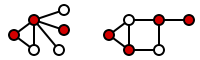
\includegraphics[width=0.4\textwidth]{../doc/img/vertex-cover.png}
\label{fig:cv}
}
\subfigure[Coberturas mínimas de vértices]{
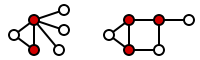
\includegraphics[width=0.4\textwidth]{../doc/img/minimum-vertex-cover.png}
\label{fig:cmv}
}
\caption{Exemplos de coberturas de vértices}
\label{fig:cv-cmv}
\end{figure}
}


\subsection{Aplicações}
\frame{
\frametitle{Definição}
\begin{itemize}
    \item Exemplo 1
    \item Exemplo 2
    \item Exemplo 3
    \item Exemplo 4
\end{itemize}
}

\subsection{Complexidade}
\frame{
\frametitle{Complexidade}
\begin{itemize}
\item Para o caso geral, encontrar a CMV de um grafo $G = (V, E)$ é um
    problema NP-Completo.

\item Um algoritmo que encontre a CMV $C$ por busca exaustiva executa
em tempo $2^{O(k)n^{O(1)}}$, onde $n = \left| V \right|$ e $k = \left|
C \right|$.

\item Utilizando a técnica de \textit{bounded search
tree algorithm}, é possível reduzir o tempo de execução para
$2^{o(k)n^{O(1)}}$.
\end{itemize}
}

\section{Algoritmos conhecidos}
\subsection{Algoritmos aproximativos}
\frame{
\frametitle{Primeiro algoritmo}
\begin{block}{primeiroAlgoritmo($G$)}
\begin{enumerate}
    \item $C \rightarrow \emptyset$
    \item while $E \ne \emptyset$
    \begin{enumerate}
        \item Escolha $e = (a,b) \in E$ aribitrariamente.
        \item $C = C \cup {a,b}$
        \item $E \rightarrow E \backslash \{e \in E : a \mbox{ ou } b \in E\}$
    \end{enumerate}
\end{enumerate}
\end{block}

\begin{itemize}
    \item Sempre acha uma solução até 2 vezes pior que a solução
        ótima.
    \item Executa em $O(V+E)$.
    \item Descoberto independentemente por~\cite{cite:simple}.
\end{itemize}
}

\frame{
\frametitle{Segundo algoritmo}
\begin{itemize}
    \item Existem algoritmos com um fator de aproximação ligeiramente
        melhores.
    \item Um algoritmo, usando técnicas avançadas e programação
    linear, é conhecido~\cite{cite:complex}. Seu fator de aproximação
    é de $2 - \Theta(\dfrac{1}{\sqrt{\log V}})$.
\end{itemize}
}

\subsection{Heurísticas}
\frame[allowframebreaks]{
\frametitle{Algoritmo guloso}
\begin{block}{Guloso($G$)}
\begin{enumerate}
    \item $C \rightarrow \emptyset$
    \item while $E \ne \emptyset$
    \begin{enumerate}
        \item Seja $v \in G : d[v] \ge d[u], \forall u \in V$
        \item $C = C \cup {v}$
        \item $E \rightarrow E \backslash \{e \in E : v \in E\}$
    \end{enumerate}
\end{enumerate}
\end{block}

O algoritmo acima parte do príncipio de escolher os vértices que têm
mais arestas incidentes a ele para o CMV, de forma a cobrir o mais
número de arestas com o menor número de vértices.

\framebreak

No entanto, este algoritmo falha mais vezes que a intuição indica.

\begin{figure}[htb]
\centering
\subfigure[Caso ótimo]{
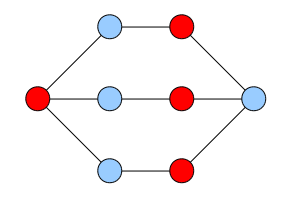
\includegraphics[width=0.4\textwidth]{../doc/img/optimal.png}
\label{fig:optimalguloso}
}
\subfigure[Solução encontrada]{
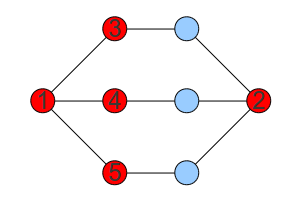
\includegraphics[width=0.4\textwidth]{../doc/img/wrong.png}
\label{fig:wrongguloso}
}
\caption{Exemplo de caso em que o algoritmo guloso falha}
\label{fig:guloso}
\end{figure}
}

\section{Heurística proposta}
\subsection{Príncipio}
\frame{
\frametitle{Príncipio}

\begin{block}{Princípio}
Se existe uma aresta $e=(u,v)$, e $d[u] = 1$,
então existe uma CMV $C$ tal que $v \in C$.
\end{block}

\begin{figure}[htb]
\centering
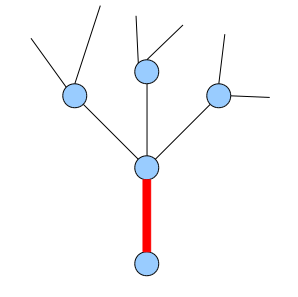
\includegraphics[width=0.3\textwidth]{../doc/img/principio.png}
\caption{Exemplo de escolha ótima local}
\label{fig:principio}
\end{figure}
}

    
    \section{Comentários finais}
    \frame{

        \frametitle{Comentários finais}

        \begin{itemize}
            \item A princípio, pode parecer que poucas aplicações se
                beneficiariam da arquitetura proposta pela Google.

            \item No entanto, aplicações que se focam na relação
            performance/preço e que não tenham estado (permitindo a
            replicação dos servidores) podem se beneficiar com o uso
            de uma arquitetura similar.

            \item Alguns exemplos incluem: servidores Web de grande
            volume e servidores de aplicações computacionalmente
            intensas, mas sem estados.
        \end{itemize}

    }

    % =================== Bibliografia ==================== %
    \appendix
    \section*{\appendixname}
    \subsection*{Referências}

    \begin{frame}[allowframebreaks]
      \frametitle{Bibliografia}
        \nocite{*}
        \bibliographystyle{amsplain}
        \bibliography{../doc/tp.bib}

    \end{frame}
\end{document}
